\begin{frame}{Challenge Submission}
\framesubtitle{Backup}
    \begin{itemize}
        \item ECG-DualNet XL utilized
        \item Pre-training on Icentia$11\si{\kilo}$
        \item Optimized training ($8000$ samples) and validation ($528$ samples) split used
    \end{itemize}
    \begin{table}[!ht]
        \centering
        \caption{Classification results of ECG-DualNet XL pre-trained on the Icentia$11$k dataset and fine-tuned on the PhysioNet dataset with optimized submission split. Metric computed on the small validation set. Four class results on the top and two class results below.}
        \begin{tabular}{>{\raggedright\arraybackslash}p{0.53\columnwidth}>{\raggedright\arraybackslash}p{0.15833\columnwidth}>{\raggedright\arraybackslash}p{0.15833\columnwidth}}
    \hline
	Model & ACC $\uparrow$ & F1 $\uparrow$ \\
	\hline
	ECG-DualNet XL & $0.8840$ & $0.8549$ \\
	\hline
\end{tabular}

        \label{tab:results_challenge}
    \end{table}
    \begin{center}
        \hspace{-0.15cm}\begin{tabular}{>{\raggedright\arraybackslash}p{0.53\columnwidth}>{\raggedright\arraybackslash}p{0.15833\columnwidth}>{\raggedright\arraybackslash}p{0.15833\columnwidth}}
    \hline
	Model & ACC $\uparrow$ & F1 $\uparrow$ \\
	\hline
	ECG-DualNet XL ($2$ class) & $0.9933$ & $0.9842$ \\
	\hline
\end{tabular}

    \end{center}
\end{frame}

\begin{frame}{Deep Double Decent}
\framesubtitle{Backup}
    \begin{figure}[!ht]
        \centering
        \vspace{-0.2cm}
        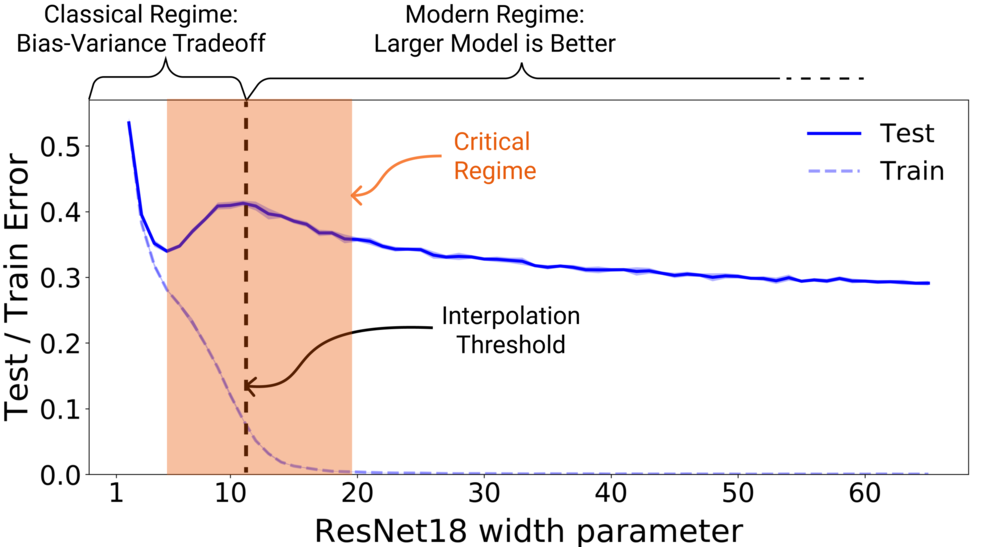
\includegraphics[width=0.6\textwidth]{artwork/deep_double_decent.png}
        \vspace{-0.2cm}
        \caption{Illustration of the deep double decent phenomenon in image classification (CIFAR-10 \& 15\% label noise). Image taken from \cite{Nakkiran2020}.}
        \label{fig:ddd}
    \end{figure}
\end{frame}